\section{Training with Missing Features}
\label{sec:training}

In this section we train a logistic regression on incomplete data with PCPG
inside the loss (Section~\ref{sec:training-pcpg}) and compare it with the usual
ways of training on incomplete data.

\subsection{Monte Carlo Inside the Loss}
\label{subsec:training-mc}

The obvious alternative to PCPG is to estimate the expectation in the loss by sampling,
\[
  \hat p = \frac{1}{S} \sum_{s=1}^{S} \sigma\!\left(w^T x^{(s)}\right),
  \qquad x^{m,(s)} \sim p(\xm \mid \xo),
\]
with new samples in every step. The samples do not depend on $w$, so the
gradient is simply the average of the gradients at the samples. The estimate
$\hat p$ itself is unbiased, but the loss is not: since $\log$ is concave,
Jensen's inequality gives
\[
  \E\left[ -\log \hat p \right] \geq -\log \E[\hat p] = -\log p ,
\]
so the Monte Carlo loss is too large on average. A second-order expansion of
$\log$ around $p$ gives the size of this bias,
\[
  \E\left[ -\log \hat p \right] + \log p \approx
  \frac{\mathrm{Var}[\hat p]}{2 p^2} = \frac{\mathrm{Var}[\sigma(z)]}{2 S p^2},
\]
where $\mathrm{Var}[\sigma(z)]$ is the variance of the prediction over the missing
features. The bias decreases like $1/S$, but it does not average out over the
steps of the optimisation. It acts as an additional penalty on how much the
prediction depends on the missing features, and it is minimised by making $w$
smaller. The Monte Carlo objective therefore has its optimum at a smaller $w$
than the marginal likelihood. For $S = 1$ the loss is the average loss over a
single random completion of every point, $\E[-\log \sigma(\pm w^T x)]$, which is
the objective of training on randomly imputed data (multiple imputation). With
growing $S$, the Monte Carlo objective moves from this objective to the
marginal likelihood.

\subsection{Compared Models}
\label{subsec:training-models}

All models are logistic regressions without intercept. They differ only in the
training points they see and in the prediction their loss is built from
(Table~\ref{tab:training-models}):
\begin{itemize}
  \item \textbf{Complete data:} an ordinary logistic regression on the complete
        training points. This is an oracle, since these points are not available
        when features are missing. It shows what training could reach without
        missing features.
  \item \textbf{Mean imputation:} an ordinary logistic regression on the training
        points with every missing feature replaced by the mean of its observed
        values.
  \item \textbf{MC, PCPG, Exact:} the marginal likelihood \eqref{eq:marginal-likelihood}
        on the incomplete training points, with the expectation estimated by Monte
        Carlo with $S$ samples, by deterministic PCPG with $M \times N$ nodes, or
        computed exactly. Exact uses the direct route for Gaussian mixtures
        (Section~\ref{subsec:gmm-direct}) with Gauss--Hermite quadrature for every
        component. It is only available for the GMM, and serves as the target of
        MC and PCPG.
\end{itemize}

\begin{table}[htb]
\centering
\small
\renewcommand{\arraystretch}{1.3}
\begin{tabular}{lll}
\hline
\textbf{Model} & \textbf{Training points} & \textbf{Prediction in the loss} \\
\hline
Complete data   & complete $x$                 & $\sigma(w^T x)$ \\
Mean imputation & $\xo$, $\xm$ filled by means & $\sigma(w^T x)$ \\
MC              & $\xo$                        & $\frac{1}{S}\sum_s \sigma(w^T x^{(s)})$ \\
PCPG            & $\xo$                        & PCPG, $M \times N$ nodes \\
Exact           & $\xo$                        & $\sum_k \tilde\pi_k(\xo) \E_{\mathcal{N}(m_k, v_k)}[\sigma(z)]$ \\
\hline
\end{tabular}
\caption{The compared models. The last three minimise the marginal likelihood
  \eqref{eq:marginal-likelihood}, the first two an ordinary logistic regression
  loss. All use the same $L_2$ penalty.}
\label{tab:training-models}
\end{table}

MC, PCPG and Exact are trained in the same way, with Adam on minibatches,
starting from $w = 0$. Complete data and mean imputation are ordinary logistic
regressions and are fit with scikit-learn, which finds their optimum exactly.

\subsection{Evaluation}
\label{subsec:training-evaluation}

Every trained $w$ is scored in three ways.
\begin{itemize}
  \item \textbf{Objective gap} $J(w) - J(w^*)$, where $J$ is the exact marginal
        likelihood \eqref{eq:marginal-likelihood} on the training points and
        $w^*$ its optimum, found by full-batch L-BFGS. It measures how well a model
        minimises the marginal likelihood, so its target is Exact. For complete
        data and mean imputation it also contains the difference between their
        objective and the marginal likelihood.
  \item \textbf{Test accuracy on incomplete points:} every model predicts with the
        exact expected prediction on test points with the same fraction of
        missing features, so the models only differ in $w$.
  \item \textbf{Test accuracy on complete points:} the accuracy of
        $\sigma(w^T x)$ on the complete test points, i.e.\ how good $w$ is as a
        classifier.
\end{itemize}
For both accuracies the target is the complete-data model, the classifier that
training could reach if no features were missing.

\subsection{Setup}
\label{subsec:training-setup}

The data are again generated with scikit-learn's \texttt{make\_classification}, with
10{,}000 samples, 8{,}000 for training and 2{,}000 for testing. In contrast to
Section~\ref{sec:weight-norm}, half of the features are informative and the
others are noise, without redundant features: with only two informative
features, almost all missing features would be irrelevant for the label. The
number of features is $d \in \{5, 10, 20, 50, 100\}$. In every training and test
point, $\lfloor \rho d \rfloor$ features are hidden at random, with
$\rho \in \{0.3, 0.5, 0.8\}$. The density is a GMM with $K = 4$ diagonal
components, fit on the incomplete training points. PCPG uses $M = 10$
Golub--Welsch nodes and $N = 32$ Gauss--Hermite nodes, and MC gets the same
budget of $S = 320$ samples per point and step. Exact uses 64 Gauss--Hermite
nodes per component. Adam runs for 100 epochs with minibatches of 1{,}024 points
and a learning rate of $0.01$.

\subsection{Results}
\label{subsec:training-results}

All results are for a single random choice of the hidden features per setting.
With 2{,}000 test points, an accuracy has a standard error of about
$0.9$ percentage points, so smaller differences in accuracy are not meaningful.

\begin{figure}[htb]
  \centering
  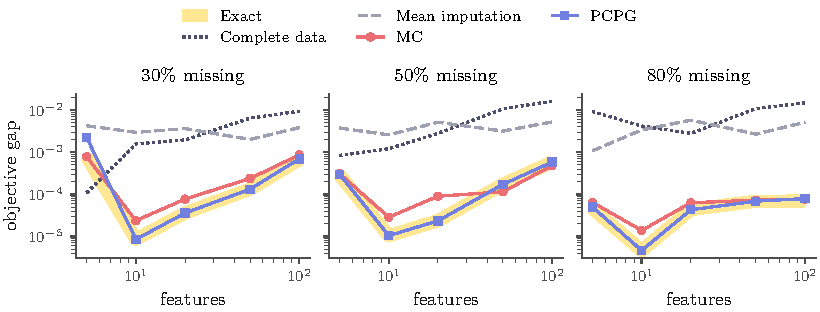
\includegraphics[width=\textwidth]{figures/train/gmm/comparison_gap.pdf}
  \caption[Objective gap of the trained classifiers]{Objective gap
    $J(w) - J(w^*)$ of the trained classifiers against the number of features $d$,
    for 30\%, 50\% and 80\% missing features. $J$ is the exact marginal likelihood
    \eqref{eq:marginal-likelihood} on the training points, and the target is the
    classifier trained with the exact expectation (yellow band). MC uses
    $S = 320$ samples, PCPG $10 \times 32$ nodes.}
  \label{fig:training-gap}
\end{figure}

\paragraph{The marginal likelihood is reached.}
Figure~\ref{fig:training-gap} shows how well every model minimises the marginal
likelihood. MC, PCPG and Exact mostly end between $5 \cdot 10^{-6}$ and
$10^{-4}$ above the optimum, complete data and mean imputation mostly between
$10^{-3}$ and $2 \cdot 10^{-2}$. The baselines minimise a different objective, so
their gap does not shrink with more training: it is the price of ignoring the
uncertainty of the missing features. PCPG follows Exact closely in almost all
settings, i.e.\ its quadrature error does not affect the training. MC lies
slightly above it, by up to $7 \cdot 10^{-5}$ for 10 and 20 features. With
$S = 320$ samples its bias $\mathrm{Var}[\sigma(z)] / (2 S p^2)$ is small, but
visible. At both ends of the range of $d$ the gaps are larger, for all three
methods including Exact, so the cause is the optimiser and not the expectation:
Adam with a fixed learning rate does not settle exactly at the optimum. At
5 features it has to reach large weights ($\lVert w^* \rVert \approx 3$), and Exact
stops $7.8 \cdot 10^{-4}$ above the optimum at 30\% missing, more than the
complete-data classifier ($1.1 \cdot 10^{-4}$). At 100 features there are many
weights, and all three stop at about $6 \cdot 10^{-4}$ for 30\% and 50\% missing.
In one setting PCPG falls behind Exact: with 5 features and 30\% missing only a
single feature is hidden, so $z \mid \xo$ is concentrated and the characteristic
function hardly decays, which is the hardest case for the fixed nodes of PCPG.
Its gap of $2.2 \cdot 10^{-3}$ is three times that of Exact.

\begin{figure}[htb]
  \centering
  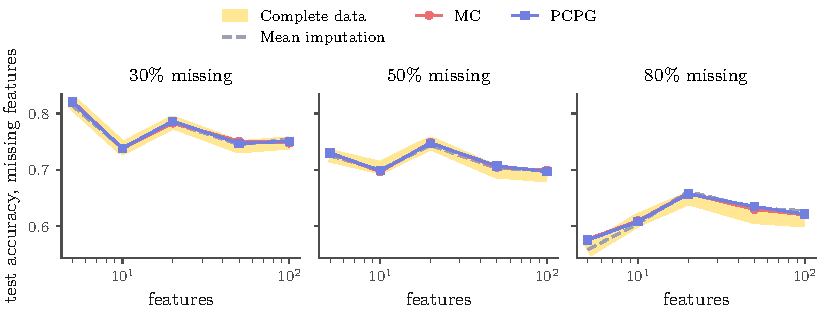
\includegraphics[width=\textwidth]{figures/train/gmm/comparison_accuracy_missing.pdf}
  \caption[Test accuracy on incomplete points]{Test accuracy on test points with
    the same fraction of missing features, every classifier with the exact
    expected prediction. The target is the classifier trained on complete data
    (yellow band).}
  \label{fig:training-accuracy-missing}
\end{figure}

\paragraph{Accuracy on incomplete test points.}
When the test points are incomplete as well
(Figure~\ref{fig:training-accuracy-missing}), all classifiers reach almost the
same accuracy at 30\% and 50\% missing. At 80\% missing, the classifiers trained
on the marginal likelihood are more accurate than the one trained on complete
data, by 2.0 percentage points at 5 features ($57.7\%$ against $55.7\%$), 1.9 at
50 features and 1.4 at 100 features. The complete-data classifier is optimal for
complete points, not for the expected prediction it is used with here, while the
marginal likelihood trains exactly for that prediction. Mean imputation lies
close to the marginal likelihood at 50 and 100 features, but 1.9 percentage
points below it at 5 features.

\begin{figure}[htb]
  \centering
  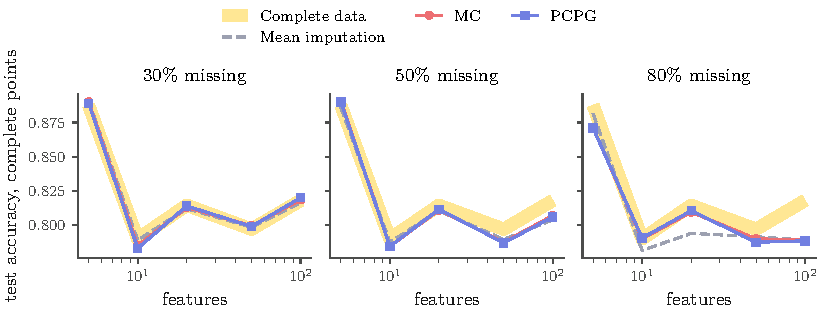
\includegraphics[width=\textwidth]{figures/train/gmm/comparison_accuracy_complete.pdf}
  \caption[Test accuracy on complete points]{Test accuracy of $\sigma(w^T x)$ on
    the complete test points, i.e.\ how good the classifier is when nothing is
    missing. The target is the classifier trained on complete data (yellow band).}
  \label{fig:training-accuracy-complete}
\end{figure}

\paragraph{Accuracy on complete test points.}
Figure~\ref{fig:training-accuracy-complete} shows how much of the classifier is
lost by training on incomplete data, measured on complete test points. At 30\%
and 50\% missing, all classifiers lie within 1.5 percentage points of the
complete-data classifier. At 80\% missing they fall behind it, by up to
$2.9$ percentage points at 100 features. Here, the classifiers trained on the
marginal likelihood are ahead of mean imputation at 10 and 20 features
($81.1\%$ against $79.4\%$ at 20 features), and level with it at 50 and 100
features. At 5 features, mean imputation is ahead by 1.1 percentage points.

\begin{figure}[htb]
  \centering
  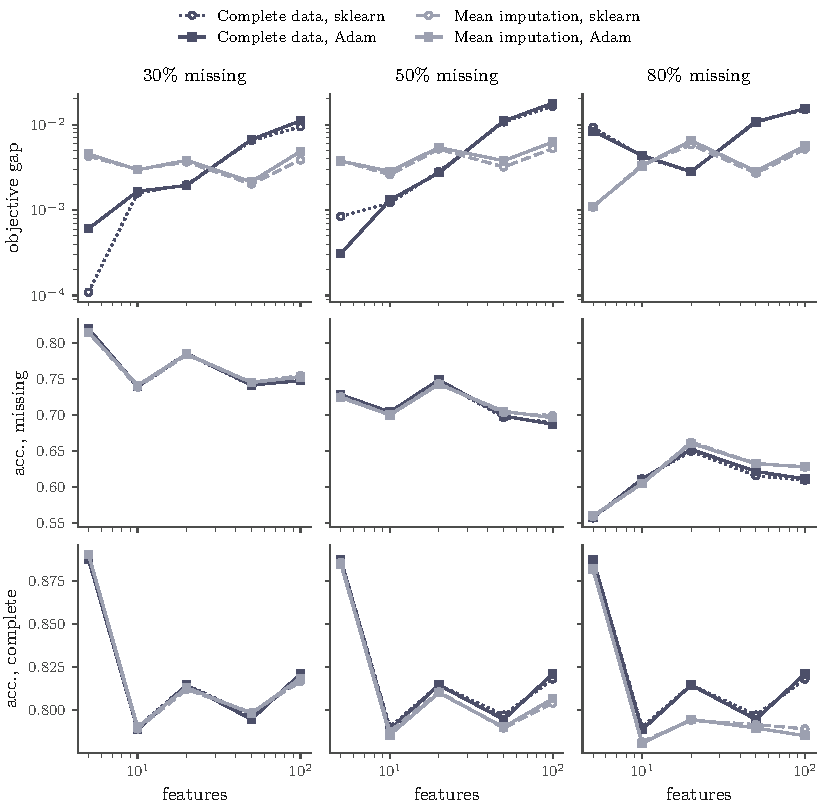
\includegraphics[width=\textwidth]{figures/train/gmm/comparison_sklearn.pdf}
  \caption[Complete data and mean imputation by scikit-learn and Adam]{The two
    ordinary logistic regressions, fit with scikit-learn (open markers) and with the
    same Adam schedule as the other models (filled markers): objective gap, and
    test accuracy on incomplete and on complete test points.}
  \label{fig:training-sklearn}
\end{figure}

\paragraph{Adam against an exact solver.}
To check that the training by Adam does not distort the comparison, we also
fit complete data and mean imputation with Adam, in the same way as MC, PCPG and
Exact (Figure~\ref{fig:training-sklearn}). Both fits give practically the same
accuracies, and the same objective gap except at 5 features, where Adam does not
reach the optimum of the logistic regression. There its gap differs from that of
scikit-learn by up to a factor of five, in both directions, since the gap is
measured on the marginal likelihood and not on the objective the two fits
minimise. This is the same limitation of the optimiser as for Exact above, and
it does not change the comparison between the models.

\paragraph{Summary.}
PCPG makes the marginal likelihood usable as a training loss: the training with
PCPG reaches the same classifier as training with the exact expectation, without
sampling and without the systematic bias of Monte Carlo. Training on the
marginal likelihood makes the classifier better suited to incomplete test
points than training on complete data, with gains of up to two percentage points
of accuracy at 80\% missing features. On complete test points, it loses less
than mean imputation at high missing rates and moderate dimensions. In terms of
accuracy, the differences between the methods are small on this data, while in
terms of the objective they are clear: only the marginal likelihood models
reach its optimum.
